% SIAM Article Template
\documentclass[review]{siamonline1116}

% Information that is shared between the article and the supplement
% (title and author information, macros, packages, etc.) goes into
% ex_shared.tex. If there is no supplement, this file can be included
% directly.

% SIAM Shared Information Template
% This is information that is shared between the main document and any
% supplement. If no supplement is required, then this information can
% be included directly in the main document.


% Packages and macros go here
\usepackage{lipsum}
\usepackage{amsfonts}
\usepackage{graphicx}
\usepackage{epstopdf}
\usepackage{algorithmic}
\ifpdf
  \DeclareGraphicsExtensions{.eps,.pdf,.png,.jpg}
\else
  \DeclareGraphicsExtensions{.eps}
\fi

%strongly recommended
\numberwithin{theorem}{section}

% Declare title and authors, without \thanks
\newcommand{\TheTitle}{An Example Article} 
\newcommand{\TheAuthors}{D. Doe, P. T. Frank, and J. E. Smith}

% Sets running headers as well as PDF title and authors
\headers{\TheTitle}{\TheAuthors}

% Title. If the supplement option is on, then "Supplementary Material"
% is automatically inserted before the title.
\title{{\TheTitle}\thanks{Submitted to the editors DATE.
\funding{This work was funded by the Fog Research Institute under contract no.~FRI-454.}}}

% Authors: full names plus addresses.
\author{
  Dianne Doe\thanks{Imagination Corp., Chicago, IL
    (\email{ddoe@imag.com}, \url{http://www.imag.com/\string~ddoe/}).}
  \and
  Paul T. Frank\thanks{Department of Applied Mathematics, Fictional
    University, Boise, ID (\email{ptfrank@fictional.edu},
    \email{jesmith@fictional.edu}).}
  \and
  Jane E. Smith\footnotemark[3]
}

\usepackage{amsopn}
\DeclareMathOperator{\diag}{diag}


%%% Local Variables: 
%%% mode:latex
%%% TeX-master: "ex_article"
%%% End: 


% Optional PDF information
\ifpdf
\hypersetup{
  pdftitle={\TheTitle},
  pdfauthor={\TheAuthors}
}
\fi

% The next statement enables references to information in the
% supplement. See the xr-hyperref package for details.

\externaldocument{ex_supplement}

% FundRef data to be entered by SIAM
%<funding-group>
%<award-group>
%<funding-source>
%<named-content content-type="funder-name"> 
%</named-content> 
%<named-content content-type="funder-identifier"> 
%</named-content>
%</funding-source>
%<award-id> </award-id>
%</award-group>
%</funding-group>



\title{Parameter Estimation for JSPAM Galactic Merger Simulations Using a Modified Metropolis-Hastings Method}
\author{Graham West, John Wallin, Zach Sinkala}


\begin{document}

\maketitle

% REQUIRED
\begin{abstract}
Gravitational N-body models can used to model the dynamical properties of interacting galaxies.  These models represent states in a six-dimensional phase space with three-dimensional projections that can observed with astronomical telescopes.  Although these models have thousands of particles, the dynamical state that describes the system can be represented with twelve dynamical parameters.
In this paper, we present the implementation and results of an MCMC-type optimization method to solve the problem of estimating these dynamical parameters for galaxy mergers. Using an adaptive Metropolis-Hastings algorithm combined with the appropriate error function, we are able to find a merger simulation of minimum error with respect to a given merger target. We also explore the connections between the convergence of the method and the sensitivity of the parameters in this system.
\end{abstract}

% REQUIRED
\begin{keywords}
non-linear dynamics, cosmology, MCMC, galaxy mergers, simulation, optimization
\end{keywords}

% REQUIRED
\begin{AMS}
  68Q25, 68R10, 68U05
\end{AMS}

\section{Introduction}
Understanding the morphology and evolution of galactic mergers is a central issue in contemporary astrophysicis--in particular, the inverse problem of tracing a merger back in time to determine its dynamical history. Due to the highly non-linear nature of galactic systems as well as limited observational knowledge of a given system's current state, this problem cannot be solved by simply reversing time in an N-body simulation, necessitating the use search algorithms which require a great number of merger simulations to fully explore the parameter space.

In order to resolve this problem, we need three things: 1) a fast simulation code, 2) an error function which accurately measures the differences between two mergers, and 3) an optimization algorithm which can minimize that error function. Step 1 was completed by Wallin et al. \cite{jspam} with the development of the simulation code entitled JSPAM. Steps 2 and 3 both will be described in this paper since an optimization problem is intimiately linked to its error function.

%(Throughout this paper, we will speak of \textit{minimizing} the fitness function since it is in the form of an error function, i.e., a low value means a high fitness.) 

In what follows, we will discuss the tools and data we had at our disposal, including JSPAM, \textit{Galaxy Zoo: Mergers} and \textit{Merger Wars}, and the SDSS and MaNGA surveys. Then--in the majority of the paper--we will examine our method of calculating the error function and the MCMC algorithm which minimizes it.   We will show how this algorithm converges on some sample systems, and explore how the sensitivity of the dynamical parameters that define our system are related to the convergence rate of the MCMC method.  Finally, we will discuss several future steps which we will take to integrate the MaNGA data into our process so that we can begin fitting real mergers.


\subsection{JSPAM}

Due to the nature of gravitation as a pair-wise interaction and the structure of galaxies being primarily a cloud of massive, interacting particles, the most direct way to simulate a merger would be to set up a full $O(n^2)$ N-body code. Approximations can be made which reduce the complexity to $O(n\hspace{1pt}$log$(n))$--hierarchical tree codes, for example--but, even this is too slow for our purposes. Due to the great quantity of simulations needed to be performed, we required a code which was $O(n)$. Thus, we used the restricted three-body JSPAM code developed by Wallin et al. \cite{jspam}.

This code makes several significant simplifications for the sake of runtime, but since the mergers are not simulated over a long time interval, accuracy is retained.  A detailed description of the code is contained in \cite{jspam}, so we will provide only a brief overview of its functionality. Within the code, galaxies themselves are comprised of two parts: a center of mass and a swarm of massless particles. The massless particles only interact with the masses of the two galaxies while the centers of mass interact with both each other and the particles.  Initially these particles are placed in a single disk of circular orbits in specified orbital plane around the center of mass of their respective galaxy.  The gravitational fields
%(say field or potential?)
around the center of masses of the galaxies are spherically symmetric.  These fields are modeled after the disk, bulge and halo potential described by Hernquist (1988?) used to model the self-consistent gravitational fields of disk galaxies.

The reference frame of the simulation is setup so that one galaxy (called the primary) is initially at the origin with zero velocity and the other galaxy (called the secondary) is given a relative position and velocity.  The equation that describes the acceleration of the ith particle is at position $r_i$ is:
% big equation needed here
\begin{equation}
\vec{a}_i = - \frac{G M_1(| \vec{r}_i - \vec{R}_1|)}{ (\vec{r}_i - \vec{R}_1)^2}\hat{r}_{i1} -
\frac{G M_2(| \vec{r}_i - \vec{R}_2|)}{ (\vec{r}_i - \vec{R}_2)^2}\hat{r}_{i2} 
\end{equation}
where $M_1(r)$ and $M_2(r)$ are the cumulative mass distributions of the two galaxies, $R_1$ and $R_2$ and the center of mass positions, and G is the universal gravitational constant.

The list of dynamical parameters which describe the merger include these relative positions and velocities, the masses of the galaxies, their radii, and their orientations in terms of altitude and azimuth (w.r.t. the $z$-axis), for a total of 14 parameters.  Since the projected position of the two galaxies are constrained by astronomical observations (x, y are always known), there are 12 free parameters in the simulations.

\begin{figure}[!h]
	\centering
	\begin{align*}
		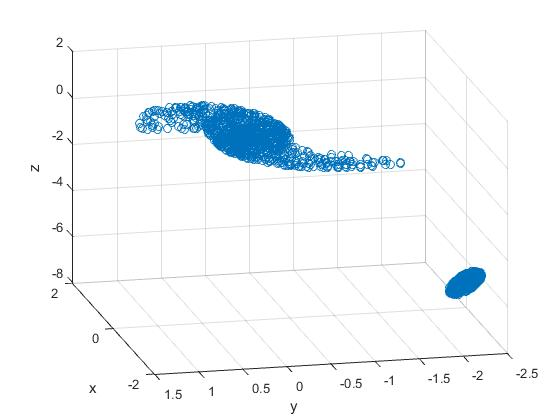
\includegraphics[scale = 0.35]{JSPAMTestPlot_xyz} & 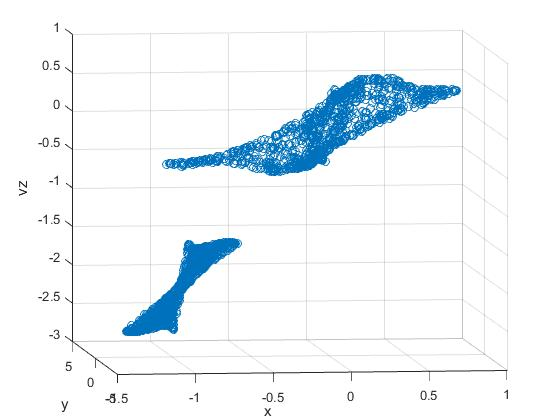
\includegraphics[scale = 0.35]{JSPAMTestPlot_xyvz}
	\end{align*}
	\caption{Final time-step of a JSPAM merger simulation (1000 particles per galaxy). Left: X-Y-Z plot. Right X-Y-Vz plot. NOTE: the graphs are viewed at two different orientations.}
\end{figure}

Given a list of \emph{final} parameters post-merger, the centers of mass are placed at their respective positions and integrated backward in time, past the point of closest approach to a fixed starting time. Then, particle positions and velocities as well as the galactic potential are then initialized. Finally, the system is integrated forward in time, with the centers of mass back to their original positions. Since the galactic potential is a fairly complicated function which must be called many times throughout a simulation, it is assumed to be spherically symmetric, pre-calculated at a set of fixed radial distances, and stored. During simulations, the value of the potential in between these radii is calculated via linear interpolation. Since the potentials are stored, they do not change over time; however, since they originate from the centers of mass, they do translate through space. In addition to the potential, JSPAM also includes a force due to dynamical friction. This phenomenon slows objects traveling through a medium of gravitating particles by causing an increase in particle density behind the object, thus increasing the gravitational force in the retrograde direction.

\subsection{Galaxy Zoo: Mergers and Merger Wars}

From a computational perspective, the problem of finding an appropriate function for comparing morphologies is a real challenge. It is difficult to find a method that is robust enough to perform on a level equivalent to that of a human. By nature, humans are excellent at pattern recognition; and where it can be difficult to ``train'' an algorithm to spot similarities between objects, humans can do it almost instinctively. For this reason, Holincheck et al. \cite{citizen} employed the help of thousands of citizen scientists to assist the \emph{Galaxy Zoo: Mergers} project in which they volunteered their pattern recognition abilities to determine best-fit models for 62 actual mergers.

The volunteers analyzed the morphologies of many thousands of simulations via a vote-based tournament scheme called the \emph{Merger Wars} algorithm. In a typical session, a volunteer is shown an image of the target (the actual merger) along with two simulations which model the target. The volunteer then chooses which simulation is most similar to the target, which counts as a ``win'' for one and a ``loss'' for the other. (They can also select neither image, thereby affording both images a loss.) Since it is entirely possible for images to be judged poorly, every simulation participates in multiple rounds of the tournament so that a bad round does not have a large impact on the results of the competition. The fitness of a particular simulation is then calculated as the percentage of ``wins'' it achieved, with the maximum being 1. Since an integral part of our research involved find an explicit mathematical fitness function for the merger morphologies, it was very useful to have the \emph{Merger Wars} data with which we could assess the validity of our own data.

\subsection{SDSS and MaNGA}

The end goal of our research is to construct an automated pipeline which can compare the morphologies of simulated mergers with images of actual mergers. Once we reach this stage, we will use the Sloan Digital Sky Survey's (SDSS) extensive catalog of observational data. Over the years, SDSS has provided many large, detailed data releases on collections of galactic mergers, the latest of which includes data from the Mapping Nearby Galaxies at APO (MaNGA) project. Thanks to the use of new observational tools, MaNGA has been able to capture spectra over the surface of nearly 2,000 galaxies, including many mergers. With this information, it is possible to derive the $z$-velocity fields and dispersions of the galaxies ($z$ being the axis from the telescope to the galaxy with positive $z$ in the direction of the telescope) and using these velocity fields, we will be able to apply our MCMC method for estimating the mergers' dynamical parameters.

\begin{figure}[!h]
	\centering
	\begin{align*}
		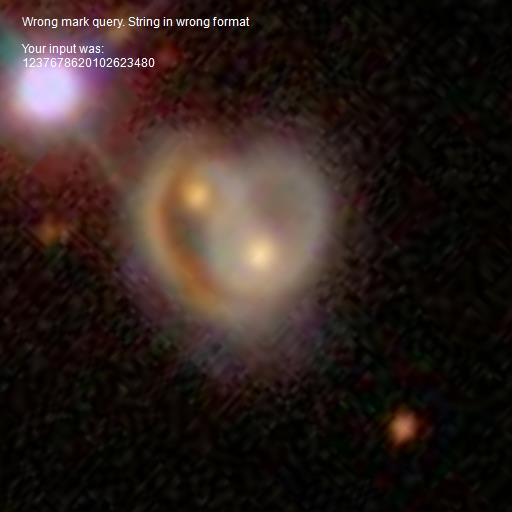
\includegraphics[scale = 0.38]{heartgalaxy} & \hspace{5mm}
		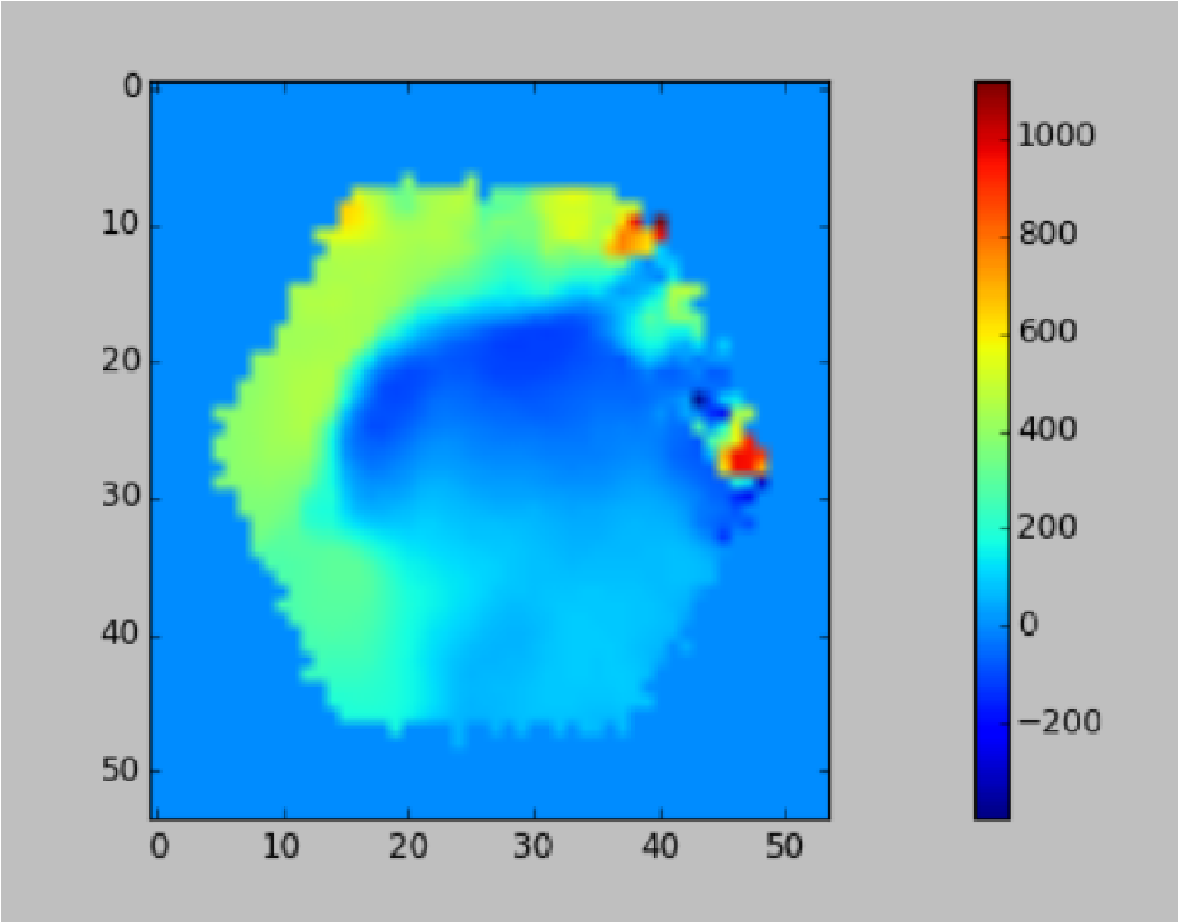
\includegraphics[scale = 0.265]{heartgalaxy_velocity}
	\end{align*}
	\caption{Visible image ($512 \times 512$ pixels) and $z$-velocity ($54 \times 54$ pixels) of a merger observed by MaNGA.}
\end{figure}

\section{Methods}

At its heart, a parameter estimation problem is essentially an optimization problem in which one minimizes a given error funciton w.r.t. a set of parameters. The two fundamental parts to the solution of such an optimization problem are 1) a meaningful error function and 2) a robust optimization algorithm. In this section, we will examine the reasoning behind the function we developed as well as the modifications we made to the canonical Metropolis-Hastings method.

\subsection{Error Function}

There are essentially two types of information which our error function must capture: particle positions and velocities. Obviously, however, we can't evalute our function on a per-particle basis because--among many reasons--once we begin using real merger targets, we will not have per-star information for them. It was very important that we kept the context of real merger targets in our minds as we experimented with the different functions because whatever we decided on in the testing phase must still be applicable to real targets. Fortunately, this restriction led us to an elegant solution to the problem. The MaNGA data is in the format of a $54 \times 54$ image for the $z$-velocity and a $512 \times 512$ image for visible light intensity. Therefore, simply binning the particle number and $z$-velocity of a simulation will give us an equivalent format.

% mention alignment

Binning the particle number is trivial; however, when binning the $z$-velocity, we must account for the opacity of gas and dust within the galaxies. To do so, we bin the velocities in 3D, averageing the values of all the particles within each bin to get its value. The equation which governs the decrease in intensity of light as it passes through a medium of density $\rho$ from $z_-$ to $z_+$ is:
\begin{equation}
	I(x,y,z_-) = I_0(x,y,z_-) \textrm{\hspace{2pt}exp}(-\kappa \int_{z_-}^{z_+} \rho(x,y,z') dz')
\end{equation}
where $I_0$ is the the actual intensity of light generated at a point and $I$ is the intensity observed after the light has passed through  Now, we use this as a kernel weighting for the velocity to map it from 2D to 3D:
\begin{equation}
	v_{2D}(x,y) = \dfrac{\int_{z_-}^{z_+}v_{3D}(x,y,z)I(x,y,z)dz}{\int_{z_-}^{z_+}I(x,y,z)dz}
\end{equation}

% discretization

\begin{figure}[!h]
	\centering
	\begin{align*}
		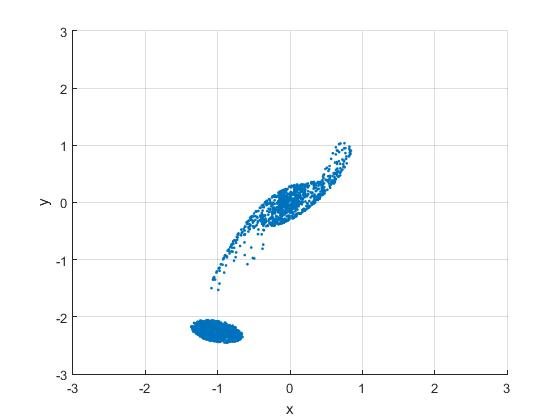
\includegraphics[scale = 0.3]{Plot_GalaxyPoints.jpg} & 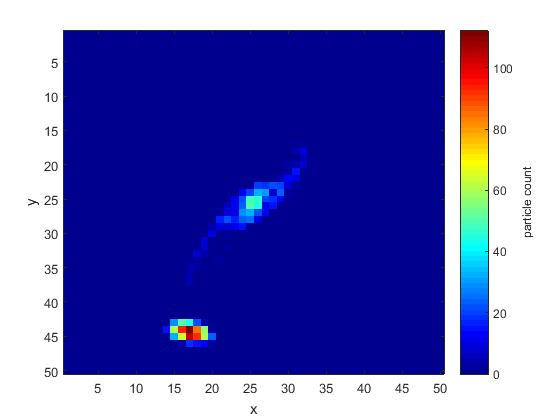
\includegraphics[scale = 0.3]{Plot_GalaxyPoints_Binned.jpg}
	\end{align*}
	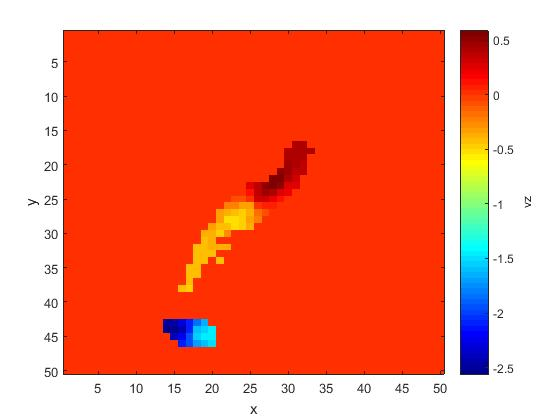
\includegraphics[scale = 0.3]{Plot_GalaxyVelocity_Binned.jpg}
		\caption{Left: a per-particle image of a merger simulation. Right: a 50x50 square-binning of the left image (high-density regions are red and low-density regions are blue). Bottom: a 50x50 square-binning of the $z$-velocities.}
\end{figure}

% plot to demonstrate opacity vs no opacity

% differentiate between the intensity of light generated at a point versus that obsevered after opacity

Having binned the simulation, we have two grids representing the $x$-$y$ distribution of particle density and $z$-velocity. We now divide the error function into two parts, one representing the similarity of the mergers' particle distributions and the other the RMS error of the $z$-velocities between them:
\begin{equation}
	f(X, X_0) = (1-OvrFrac) \cdot RMS
\end{equation}
where,
\begin{equation}
	OvrFrac = \dfrac{A_{X \cap X_0}}{A_{X}+A_{X_0}-A_{X \cap X_0}}
\end{equation}
and
\begin{equation}
	RMS^2 = \dfrac{1}{A_{X \cap X_0}}\sum_{k}^{} w_k|v_{X,k}-v_{X_0,k}|^2
\end{equation}
In these equations, $X$, $X_0$, and $X \cap X_0$ are indices referring to the \textit{simulation}, \textit{target}, and their intersection, respectively.  So, $A_{X}$ is the number of \textit{simulation} bins with particles present, $A_{X_0}$ the number of \textit{target} bins, and $A_{X \cap X_0}$ the number of \textit{overlapping} bins they share. The overlap fraction, $OvrFrac$, is the fraction of bins/pixels/area in which both the simulation and the target have particles present. $RMS$ is the weighted root-mean-squared error between the velocity fields only calculated over the overlapping bins and normalized by the number of overlapping bins (thus, $w_k = 1$ if the pixels overlap, $w_k = 0$ otherwise).

% what order to put these next two paragraphs in???
We experimented with different weighting schemes...

% converse is the wrong word
It is important to have both the overlap and RMS terms in the function. Consider the fact that morphologically similar mergers will have have high overlap and low velocity error, but the converse of this statement is not necessarily true. If the overlap is high, there is a proability that the velocity error could still be large, or vice versa. This probability is decreased if we include both velocity and overlap in the calculation.

\subsection{Adaptive Metropolis-Hastings}

% say something about the jump_sigma of the different params before talking about adaptive

Due to the chaotic nature of the merger system, the error lanscape of the parameters space is incredibly complicated, having countless local maxima and minima. Consequently, any naive gradient-based optimization scheme would be utterly unreliable. Therefore, we chose a more robust MCMC method called the Metropolis-Hastings algorithm. Given an initial set of parameter values, this method applies random--in our case normally-distributed--perturbations to the parameters. Each parameter $i$ has its own specified $\sigma_i$ for its associated distribution. At each subsequent step, the perturbations are accepted with probability $\alpha$, given by:
\begin{equation}
	\alpha(X', X) = \textrm{min}(1, \dfrac{P(X',X_0)}{P(X,X_0)})
\end{equation}
where $X'$ is the current, pperturbed simulation and $X$ is last previously accepted simulation and $P$ is given by its logairthm:
\begin{equation}
	\textrm{log}(P(X,X_0)) = \dfrac{1}{2}\textrm{log}(2 \pi \Delta^2) + \dfrac{f(X,X_0)^2}{2 \Delta^2}
\end{equation}
where $\Delta$ is a value representing the scale of the error. Also, the larger $\Delta$ becomes, the more relaxed the method will be to accept poorer simulations. In the canonical algorithm, the $\sigma_i$ values are fixed; however, we included additional functionality to allow them to adapt if multiple simulations are consequtively rejected. Let $\sigma_{i,j}$ be the $\sigma$ value for the $i$-th parameter after $j$ consequtive rejections. Then,
\begin{equation}
	\sigma_{i,j} = 
	\begin{cases} 
		\sigma_i & j \hspace{2pt} \textrm{mod} \hspace{2pt} 3 = 0 \\
		\sigma_i \cdot  M_j & j \hspace{2pt} \textrm{mod} \hspace{2pt} 3 = 1 \\
		\sigma_i \cdot  m_j & j \hspace{2pt} \textrm{mod} \hspace{2pt} 3 = 2
	\end{cases}
\end{equation}
where,
\begin{gather}
	M_j = (1+a)^{(j+2)/3} \\
	m_j = (1-b)^{(j+1)/3}
\end{gather}
and $0<a,b<1$. These two factors serve to alternate between increasing, decreasing, and resetting the $\sigma$ values so that the MCMC can escape local minima and fall into a thin global minimum quicker.

% maybe a diagram to explain

%Everything described up to this point can be found in the canonical Metropolis-Hastings algorithm; however, due to the chaotic nature of our error function, we decided to add some extra functionality to assist the convergence of the algorithm. In the canonical algorithm, the $\sigma$ values for the parameter perturbations are fixed, but 





\section{Testing, Results, and Analysis}
Since MCMC is stochastic, individual runs tell us nothing about its convergibility. We must run many tests and calculate statistics on the collective results. Therefore, our method of testing consisted of running many instances of the MCMC in parallel, all with the same target and initial parameters, but allowing different paths through parameter space. We let the MCMC run for a fixed number of steps and determined if a run converged based on whether it reached a specified error threshold. We would then generate numerous plots and statistics with which we could determine how successful the runs were.

During testing, our binning resolution ranged between 15$\times$15 to 54$\times$54 and particle numbers were between 1,000 and 10,000 per galaxy. 









\section{Conclusions}





\section*{Acknowledgments}
We would like to acknowledge the assistance of volunteers in putting
together this example manuscript and supplement.

\bibliographystyle{siamplain}
\bibliography{references}



\begin{thebibliography}{10}

\bibitem{citizen} A. Holincheck, J. Wallin, K. Borne, L. Fortson, C. Lintott, A M. Smith, S. Bamford, W. Keel, and M. Parrish, ``Galaxy Zoo: Mergers - Dynamical Models of Interacting Galaxies.'' \textit{MNRAS}, (2016). Vol. 459, Is. 1, 720-745.

\bibitem{galaxyFE} H. Mo, F. Bosch, and S. White, \textit{Galaxy Formation and Evolution}, 2010, Cambridge University Press.

\bibitem{jspam} J. Wallin, A. Holincheck, and A. Harvey, ``JSPAM: A restricted three-body code for simulating interacting galaxies.'' \textit{Astronomy and Computing} 16, (2016). 26-33.


\end{thebibliography}


\end{document}




